%!TEX program = xelatex 
\documentclass{standalone}%opcao draft remove os links
\usepackage{amssymb,amsmath,amsfonts,amsthm,amstext,pxfonts}
\usepackage{graphicx}
\usepackage[usenames,dvipsnames]{xcolor}
\usepackage{subfigure}
\usepackage{tikz,tikz-3dplot,tkz-euclide,circuitikz,siunitx,pstricks-add,pst-coil,pst-3dplot}
\usepackage{pst-plot,pst-func,pst-eucl,pst-solides3d}
\usetkzobj{all}
\usetikzlibrary{scopes}
\usetikzlibrary{through}
\usetikzlibrary{lindenmayersystems}
\usetikzlibrary[shadings]
\usetikzlibrary{arrows}
\usetikzlibrary{intersections,positioning}

\newcommand{\norm}[1]{\left\Vert{#1}\right\Vert}
\newcommand{\eq}{=}

\begin{document}
    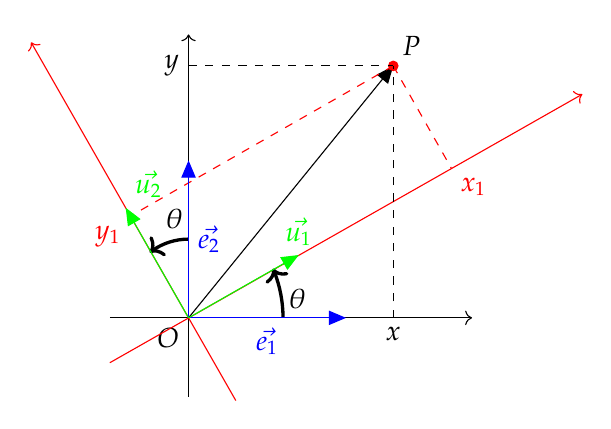
\begin{tikzpicture}[scale=2]%vetor no plano
        \coordinate[label=below left:$O$] (A) at (0,0);
        \coordinate (W) at (1.3,1.6);
        %defini\c{c}\~ao das coordenadas dos eixos cartesianos
        \coordinate (F) at (-0.5,0);
        \coordinate (G) at (0,-0.5);
        \coordinate (X) at (1.8,0);
        \coordinate (Y) at (0,1.8);
        \coordinate (F1) at (-0.5,-0.285);%y=0,57x
        \coordinate (G1) at (0.3,-0.525);%y=-1,75x
        \coordinate (X1) at (2.5,1.42);%y=0,57x
        \coordinate (Y1) at (-1,1.75);%y=-1,75x
        % Styles
        \tikzstyle{axes}=[]

        \begin{scope}[style=axes]%constr\'oi os eixos cartesianos
            \draw[->] (F) -- (X);
            \draw[->] (G) -- (Y);
            \draw[->,color=red] (F1) -- (X1);
            \draw[->,color=red] (G1) -- (Y1);
        \end{scope}

        \draw [->,black,very thick](A) +(0:.6cm) arc (0:23:.8cm);
        \node at ($(A)+(10:7mm)$) {$\theta$};
        \draw [->,black,very thick](0,0.5) +(.4cm:0) arc (90:128:.4cm);
        \node at ($(0,0.5)+(125:1.6mm)$) {$\theta$};
        \draw[->,>=triangle 45] (A)--(W)
        node[at end,above right]{$P$};
        \draw [fill,color=red] (W) circle [radius=0.03];
        \draw[dashed,red] (W) -- ($(A)!(W)!(X1)$)
        node[at end,below right]{$x_1$};
        \draw[dashed,red] (W) -- ($(A)!(W)!(Y1)$)
        node[at end,below left]{$y_1$};
        \draw[dashed,color=black] let \p1 = (W) in (\x1,0) -- (\x1,\y1)
        node[at start, below]{$x$};
        \draw[dashed,color=black] let \p1 = (W) in (0,\y1) -- (\x1,\y1)
        node[at start, left]{$y$};
        \draw[->,>=triangle 45,color=blue] (0,0) -- (1,0)
        node[midway, below]{$\vec{e_1}$};
        \draw[->,>=triangle 45,color=blue] (0,0) -- (0,1)
        node[midway, right]{$\vec{e_2}$};
        \draw[->,>=triangle 45,color=green] (0,0) -- (0.7,0.399)%y=0,57x
        node[at end, above]{$\vec{u_1}$};
        \draw[->,>=triangle 45,color=green] (0,0) -- (-0.399,0.699)%y=-1,75x
        node[at end, above right]{$\vec{u_2}$};
    \end{tikzpicture}
\end{document}